% Comparación cartesiano / cilíndrico / esférico
\documentclass[border=5pt]{standalone}
\usepackage{tikz}
\usetikzlibrary{arrows.meta, calc}
\begin{document}
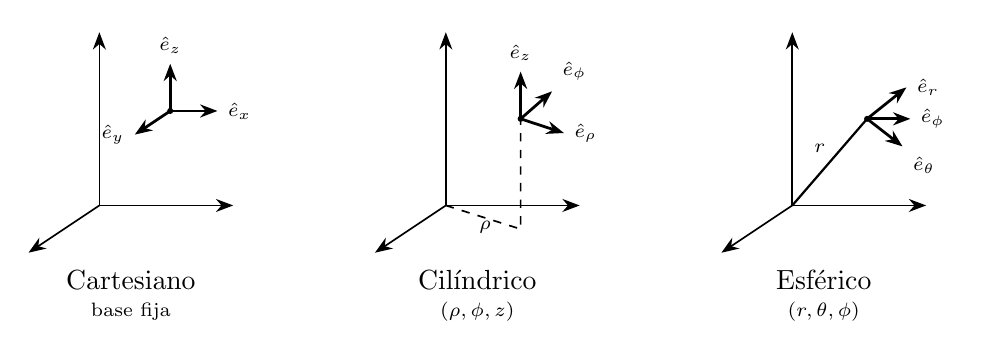
\begin{tikzpicture}[>={Stealth[length=2.2mm]}, line width=0.6pt]
  % ===== Cartesiano =====
  \begin{scope}
    \draw[->] (0,0)--(-0.9,-0.6); \draw[->] (0,0)--(1.7,0); \draw[->] (0,0)--(0,2.2);
    \coordinate (P) at (0.9,1.2); \fill (P) circle (1.1pt);
    \draw[->, line width=1pt] (P)--($(P)+(0.6,0)$) node[right]{\scriptsize$\hat e_x$};
    \draw[->, line width=1pt] (P)--($(P)+(-0.45,-0.3)$) node[left]{\scriptsize$\hat e_y$};
    \draw[->, line width=1pt] (P)--($(P)+(0,0.6)$) node[above]{\scriptsize$\hat e_z$};
    \node at (0.4,-0.95){Cartesiano};
    \node[font=\scriptsize] at (0.4,-1.35){base fija};
  \end{scope}
  % ===== Cilíndrico =====
  \begin{scope}[xshift=4.4cm]
    \draw[->] (0,0)--(-0.9,-0.6); \draw[->] (0,0)--(1.7,0); \draw[->] (0,0)--(0,2.2);
    \coordinate (F) at (0.95,-0.3); \coordinate (P) at (0.95,1.1);
    \draw[dashed] (0,0)--(F)--(P); \fill (P) circle (1.1pt);
    \node[font=\scriptsize] at (0.5,-0.28){$\rho$};
    \draw[->, line width=1pt] (P)--($(P)+(0.55,-0.18)$) node[right]{\scriptsize$\hat e_\rho$};
    \draw[->, line width=1pt] (P)--($(P)+(0.4,0.35)$) node[above right]{\scriptsize$\hat e_\phi$};
    \draw[->, line width=1pt] (P)--($(P)+(0,0.6)$) node[above]{\scriptsize$\hat e_z$};
    \node at (0.4,-0.95){Cilíndrico};
    \node[font=\scriptsize] at (0.4,-1.35){$(\rho,\phi,z)$};
  \end{scope}
  % ===== Esférico =====
  \begin{scope}[xshift=8.8cm]
    \draw[->] (0,0)--(-0.9,-0.6); \draw[->] (0,0)--(1.7,0); \draw[->] (0,0)--(0,2.2);
    \coordinate (P) at (0.95,1.1); \draw[line width=0.8pt] (0,0)--(P); \fill (P) circle (1.1pt);
    \node[font=\scriptsize] at (0.35,0.72){$r$};
    \draw[->, line width=1pt] (P)--($(P)+(0.5,0.4)$) node[right]{\scriptsize$\hat e_r$};
    \draw[->, line width=1pt] (P)--($(P)+(0.45,-0.35)$) node[below right]{\scriptsize$\hat e_\theta$};
    \draw[->, line width=1pt] (P)--($(P)+(0.55,0)$) node[right]{\scriptsize$\hat e_\phi$};
    \node at (0.4,-0.95){Esférico};
    \node[font=\scriptsize] at (0.4,-1.35){$(r,\theta,\phi)$};
  \end{scope}
\end{tikzpicture}
\end{document}
